\section{Q4 (bonus): SVMs and clustering on one fixed representation}
\label{sec:q4}

\textbf{Representation.} The 1024-d bottleneck code of the Q3(b) denoising autoencoder, frozen. Among the Q3
encoders it has the highest \emph{validation} linear-probe accuracy (0.553), so it is chosen without test
data; it was trained without labels, which keeps the clustering in (c) genuinely unsupervised. Codes are
standardised with the mean and standard deviation of the 45k training codes and never changed afterwards.
\textbf{Subset.} A kernel SVM on 45k$\times$1024 is slow (one RBF fit on 10k points takes 2--4 minutes), so a
stratified subset of 10{,}000 training images (1{,}000 per class, seed 242003) was drawn and saved
\emph{before any SVM was fitted}; every SVM uses it. Validation is the full 5k split and test the full 10k set.

\subsection{(a) Effect of C and the kernel}
We use scikit-learn's \texttt{SVC} (libsvm, one-vs-one)~\cite{cortes1995support,pedregosa2011scikit} with
$C\in\{10^{-3},\dots,10^{2}\}$ (six values, five orders of magnitude; $10^{-3}$ was added after the linear kernel
selected the lower edge of the first grid) and three kernels: linear, RBF ($\gamma=1/(d\,\mathrm{Var}(x))$) and
polynomial of degree 3 ($\gamma$ as for RBF, $c_0=1$). Table~\ref{tab:q4sweep} gives the full sweep and
Fig.~\ref{fig:q4sweep} the curves.

\begin{table}[t]
\centering
\small
\begin{tabular}{@{}l@{\hspace{3pt}}cccccc@{}}
\toprule
& \multicolumn{6}{c}{$C$} \\
\cmidrule(l){2-7}
Kernel / metric & $10^{-3}$ & $10^{-2}$ & $10^{-1}$ & $1$ & $10$ & $10^{2}$ \\
\midrule
Linear\hfill train & .573 & .681 & .832 & .954 & .997 & 1.00 \\
\hfill val & .456 & \textbf{.467} & .438 & .422 & .409 & .406 \\
\hfill SV & .905 & .853 & .823 & .807 & .801 & .799 \\
\midrule
RBF\hfill train & .324 & .324 & .477 & .841 & .998 & 1.00 \\
\hfill val & .295 & .295 & .405 & .512 & \textbf{.539} & .539 \\
\hfill SV & 1.00 & 1.00 & .989 & .953 & .965 & .964 \\
\midrule
Poly-3\hfill train & .359 & .489 & .753 & .974 & 1.00 & 1.00 \\
\hfill val & .340 & .429 & .509 & \textbf{.531} & .518 & .516 \\
\hfill SV & 1.00 & .988 & .942 & .928 & .921 & .920 \\
\bottomrule
\end{tabular}
\caption{Q4(a). Train accuracy (10k subset), validation accuracy and fraction of training points that are
support vectors, for every setting. Bold: best $C$ per kernel on validation.}
\label{tab:q4sweep}
\end{table}

\begin{figure*}[t]
\centering
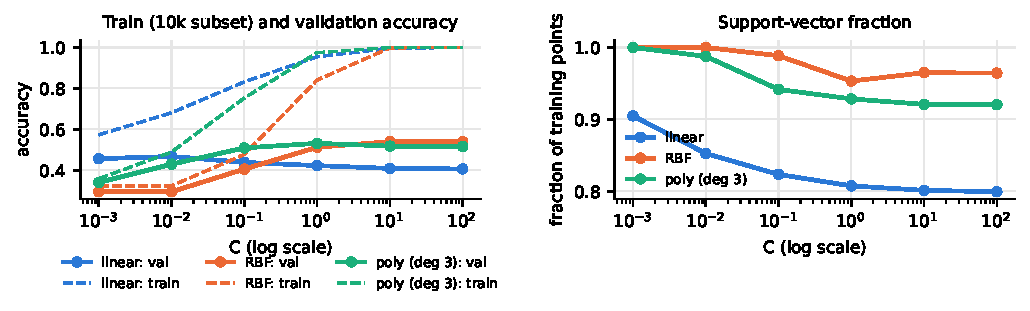
\includegraphics[width=\textwidth]{q4_sweep}
\caption{Q4(a). Left: validation (solid) and train (dashed) accuracy against $C$. Right: support-vector
fraction against $C$.}
\label{fig:q4sweep}
\end{figure*}

\textbf{Under- and overfitting.} Small $C$ means strong regularisation. RBF and polynomial kernels at
$C\le10^{-2}$ underfit badly (train 0.32--0.49, validation close to train) and every training point is a
support vector: with a tiny $C$ all points violate the margin and the solution is close to a weighted vote of
the whole training set. The linear kernel shows the opposite failure. In 1024 dimensions with 10k points it
reaches 100\% train accuracy at $C=100$, but validation falls monotonically after $C=10^{-2}$ (0.467 to 0.406):
the extra flexibility fits the training subset without transferring. The RBF kernel improves up to $C=10$ and
then flattens; once it separates the training set, a larger $C$ no longer changes the solution (same SV
fraction, same validation accuracy). The polynomial kernel peaks at $C=1$ and loses 1.5 points beyond it, a mild
overfit. The support-vector fraction stays at 0.80--1.00 throughout: the classes overlap heavily in this code,
so most points lie on or inside some pairwise margin. Its decrease with $C$ marks the move out of the
underfitting regime, but it does not predict validation accuracy (the linear kernel has the fewest support
vectors and generalises worst).

\textbf{Selection.} RBF with $C=10$ has the best validation accuracy (0.539; $C=100$ ties at 0.539). It was refit
on the same subset and evaluated once on the test set: \textbf{0.528}.

\subsection{(b) Difficult class pairs}
The three pairs with the most test confusions of the selected SVM are cat--dog (392), automobile--truck (341)
and bird--deer (288). For each pair, Fig.~\ref{fig:q4pairs} shows the four training support vectors of each class
closest to that pair's one-vs-one boundary and the eight test images of the two classes with the smallest
$|f|$, where $f$ is the pair decision score (positive = first class).

\begin{figure*}[t]
\centering
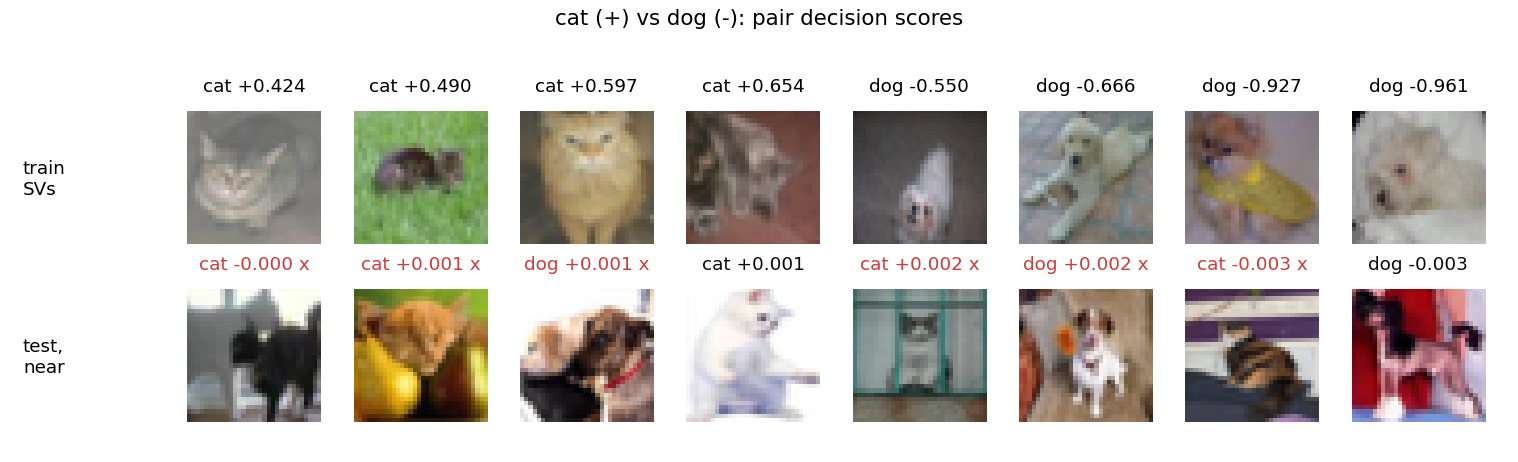
\includegraphics[width=0.82\textwidth]{q4b_pair_cat_dog}\\[-2pt]
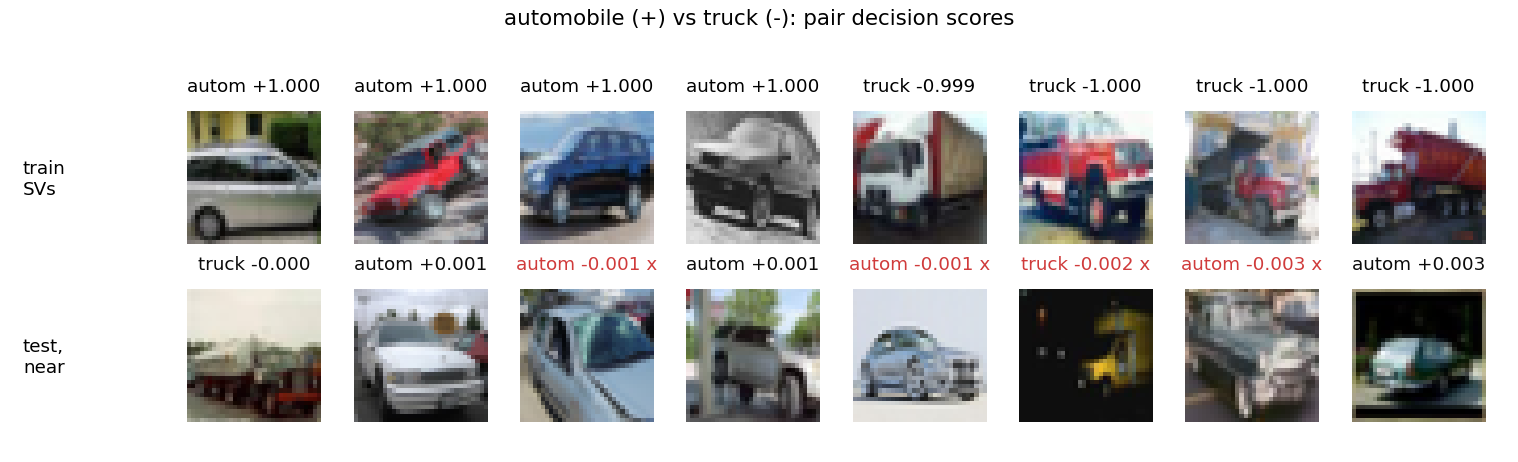
\includegraphics[width=0.82\textwidth]{q4b_pair_automobile_truck}\\[-2pt]
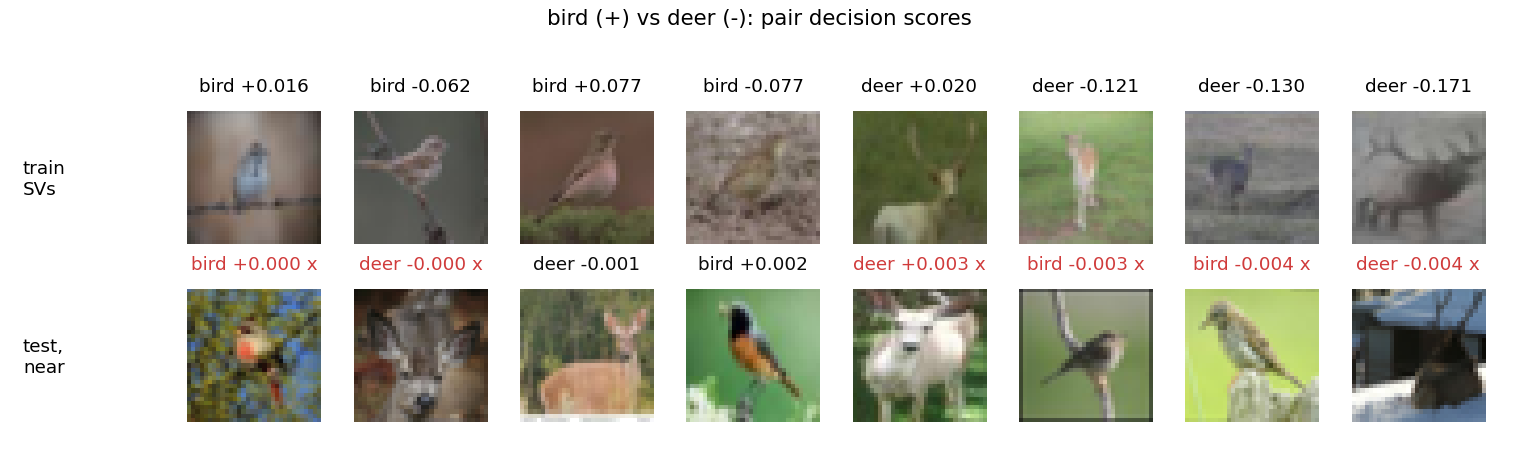
\includegraphics[width=0.82\textwidth]{q4b_pair_bird_deer}
\caption{Q4(b). Per pair, top row: training support vectors closest to the pair boundary; bottom row: test
images nearest the boundary, with the pair decision score. Red ``x'': misclassified by the 10-class SVM.}
\label{fig:q4pairs}
\end{figure*}

\begin{table}[t]
\centering
\small
\resizebox{\columnwidth}{!}{%
\begin{tabular}{@{}lcccc@{}}
\toprule
Pair & Confusions & Pair acc. & Sep.\ ratio & Pair SV frac. \\
\midrule
cat--dog & 392 & 0.634 & 0.015 & 0.95 \\
automobile--truck & 341 & 0.771 & 0.027 & 0.92 \\
bird--deer & 288 & 0.703 & 0.017 & 0.84 \\
\midrule
median of 45 pairs & -- & -- & 0.064 & -- \\
frog--ship (easiest) & 28 & 0.947 & 0.165 & -- \\
\bottomrule
\end{tabular}}
\caption{Q4(b). Test confusions (both directions), accuracy of the pair classifier on the test images of the two
classes, separation ratio (squared distance of class means over mean within-class spread, training codes) and
fraction of the pair's training points that are its support vectors.}
\label{tab:q4pairs}
\end{table}

\textbf{Errors and geometry.} In all three pairs many of the test images nearest the boundary are errors
(6, 4 and 6 of 8). The images explain the geometry. Near the cat--dog boundary are medium-sized furry animals in
the middle of the frame with grey, white or ginger fur; colour, pose and background, which the code encodes
well, do not separate them. The automobile--truck boundary is populated by silver and white vehicles seen from
the side or front, often on plain backgrounds, and dark night images. Bird and deer support vectors are small
brown or grey animals on brown and green natural backgrounds, and they sit deep inside the margin
($|f|<0.2$). Quantitatively (Tab.~\ref{tab:q4pairs}), the class means of these pairs are two to four times closer,
relative to their spread, than for a median pair, and 84--95\% of their training points are support vectors of
the pair classifier, so the boundary has to be supported by nearly the whole pair: the classes overlap instead of
being separated by a gap. Over all 45 pairs the separation ratio and the number of test confusions have a
Spearman correlation of $-0.83$, so the SVM's errors follow the geometry of the representation closely.

\subsection{(c) Clustering the same representation}
\textbf{Method and selection.} $k$-means ($k$-means++, 10 restarts) and diagonal Gaussian mixtures (3 restarts)
with $k\in\{5,10,15,20,30\}$ were fitted on the 45k training codes without labels. The choice used validation
data only: $k$-means with $k=10$ has the highest validation ARI~\cite{hubert1985comparing} (0.062; GMM at most
0.053). NMI was not used for the choice because it keeps increasing with $k$ (0.077 to 0.131). Validation
silhouettes are close to zero or negative for every candidate, a first sign that the code has little cluster
structure. The final model is the one fitted on the training codes; test codes are assigned with it and the test
labels are used only afterwards.

\begin{figure}[t]
\centering
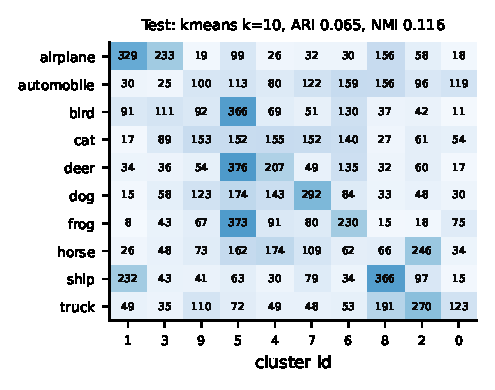
\includegraphics[width=\columnwidth]{q4_contingency}
\caption{Q4(c). Test cluster-to-class contingency table ($k$-means, $k=10$), clusters ordered by majority
class.}
\label{fig:q4cont}
\end{figure}

\textbf{Test result.} ARI 0.065 and NMI 0.116 (Fig.~\ref{fig:q4cont}), against 0.528 accuracy for the SVM. The
clusters follow colour and background more than class: one cluster collects airplanes and ships (329 and 232,
blue sky or water), another birds, deer and frogs (366, 376, 373, green and brown scenery).

\textbf{Where classification and clustering disagree.} The clearest case is \emph{automobile}. For the SVM it is
the easiest class (test recall 0.668, the highest of the ten). For the clustering it is, together with cat, the
least coherent: its largest cluster holds only 15.9\% of the automobile test images, and the row is spread over
all ten clusters (25 to 159 images each). At the pair level, the one-vs-one SVM separates automobile from cat
with 0.905 accuracy on their test images, whereas a vote in which every cluster is labelled with the majority of
the two classes among its members reaches only 0.631, and 85\% of the automobile and cat test images sit in
clusters where both classes make up at least a quarter. The same holds for automobile--horse (0.923 vs 0.658)
and automobile--dog (0.937 vs 0.675). Cars come in every colour and on every background, so colour-driven
clusters break them up, yet the code still contains directions that separate them from animals, and a supervised
RBF SVM finds them. A class can be separable without being compact, and clustering only sees the second
property. No pair goes the other way; the closest is cat--dog, where both are near chance (0.634 vs 0.584).
